\documentclass{article}
\usepackage{tikz}
\usetikzlibrary{graphs,intersections,math,animations}

\begin{document}

\begin{figure}
  \begin{center}
    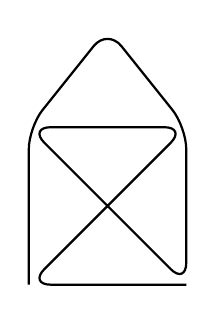
\begin{tikzpicture}
      \draw[thick,rounded corners=8pt]
      (0,0) -- (0,2) -- (1,3.25) -- (2,2) -- (2,0) -- (0,2) -- (2,2) -- (0,0) -- (2,0);
    \end{tikzpicture}
  \end{center}
  \caption{}
  \label{fig:}
\end{figure}

\begin{figure}
  \begin{center}
    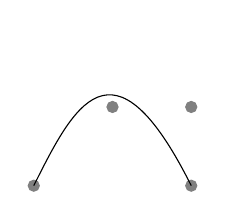
\begin{tikzpicture}
    \filldraw [gray] (0,0) circle [radius=2pt]
    (1,1) circle [radius=2pt] (2,1) circle [radius=2pt] (2,0) circle [radius=2pt];
      \draw (0,0) .. controls (0.5,1) and (1,2) .. (2,0);
    \end{tikzpicture}
  \end{center}
  \caption{}
  \label{fig:}
\end{figure}

\begin{figure}
  \begin{center}
    \begin{tikzpicture}
      \draw (-1.5,0) -- (1.5,0);
      \draw (0,-1.5) -- (0,1.5);
      \draw (-1,0) .. controls (-1,0.555) and (-0.555,1) .. (0,1)
                   .. controls (0.555,1) and (1,0.555) .. (1,0);
\end{tikzpicture}
  \end{center}
  \caption{}
  \label{fig:}
\end{figure}

\begin{figure}
  \begin{center}
    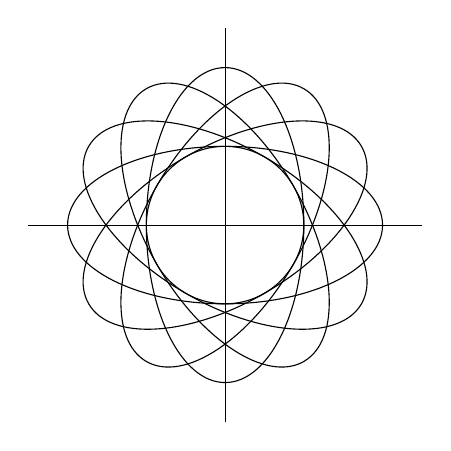
\begin{tikzpicture}
      \draw (-2.5,0) -- (2.5,0);
      \draw (0,-2.5) -- (0,2.5);
      \draw (0,0) circle[radius=1];

      \draw[rotate=0] (0,0) ellipse[x radius=2, y radius=1];
      % \draw[rotate=30] (0,0) ellipse[x radius=2, y radius=1];
      % \draw[rotate=60] (0,0) ellipse[x radius=2, y radius=1];
      % \draw[rotate=90] (0,0) ellipse[x radius=2, y radius=1];
      % \draw[rotate=120] (0,0) ellipse[x radius=2, y radius=1];
      % \draw[rotate=150] (0,0) ellipse[x radius=2, y radius=1];
      % \draw[rotate=180] (0,0) ellipse[x radius=2, y radius=1];

      \draw[rotate=210] (0,0) ellipse[x radius=2, y radius=1];
      \draw[rotate=240] (0,0) ellipse[x radius=2, y radius=1];
      \draw[rotate=270] (0,0) ellipse[x radius=2, y radius=1];
      \draw[rotate=300] (0,0) ellipse[x radius=2, y radius=1];
      \draw[rotate=330] (0,0) ellipse[x radius=2, y radius=1];
\end{tikzpicture}
  \end{center}
  \caption{}
  \label{fig:}
\end{figure}

\begin{figure}
  \begin{center}
    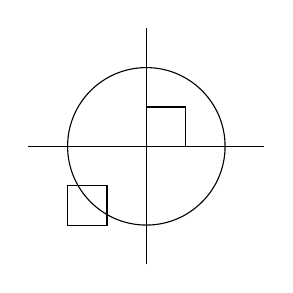
\begin{tikzpicture}
    \draw (-1.5,0) -- (1.5,0);
    \draw (0,-1.5) -- (0,1.5);
    \draw (0,0) circle [radius=1cm]; \draw (0,0) rectangle (0.5,0.5); \draw (-0.5,-0.5) rectangle (-1,-1);
    \end{tikzpicture}
  \end{center}
  \caption{}
  \label{fig:}
\end{figure}

\begin{figure}
  \begin{center}
    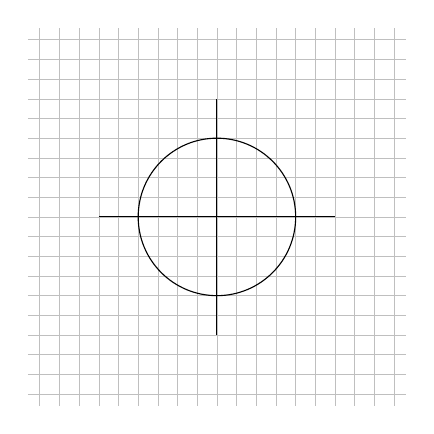
\begin{tikzpicture}
    \draw[step=.25cm,lightgray,very thin] (-2.4,-2.4) grid (2.4,2.4);
    \draw (-1.5,0) -- (1.5,0);
    \draw (0,-1.5) -- (0,1.5);
    \draw (0,0) circle [radius=1cm];
    \end{tikzpicture}
  \end{center}
  \caption{}
  \label{fig:}
\end{figure}

\begin{figure}
  \begin{center}
    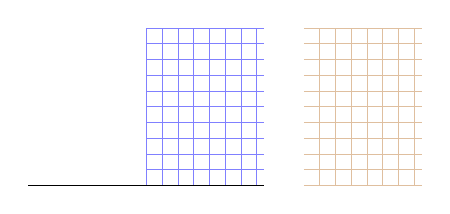
\begin{tikzpicture}[
      Karl's grid/.style ={help lines,step=0.2,color=#1!50},
      Karl's grid/.default=blue
    ]
    \draw[Karl's grid]     (0,0) grid (1.5,2);
    \draw[Karl's grid=brown] (2,0) grid (3.5,2);
    \draw (-1.5,0) -- (1.5,0);
    \end{tikzpicture}
  \end{center}
  \caption{}
  \label{fig:}
\end{figure}


\begin{figure}
  \begin{center}
    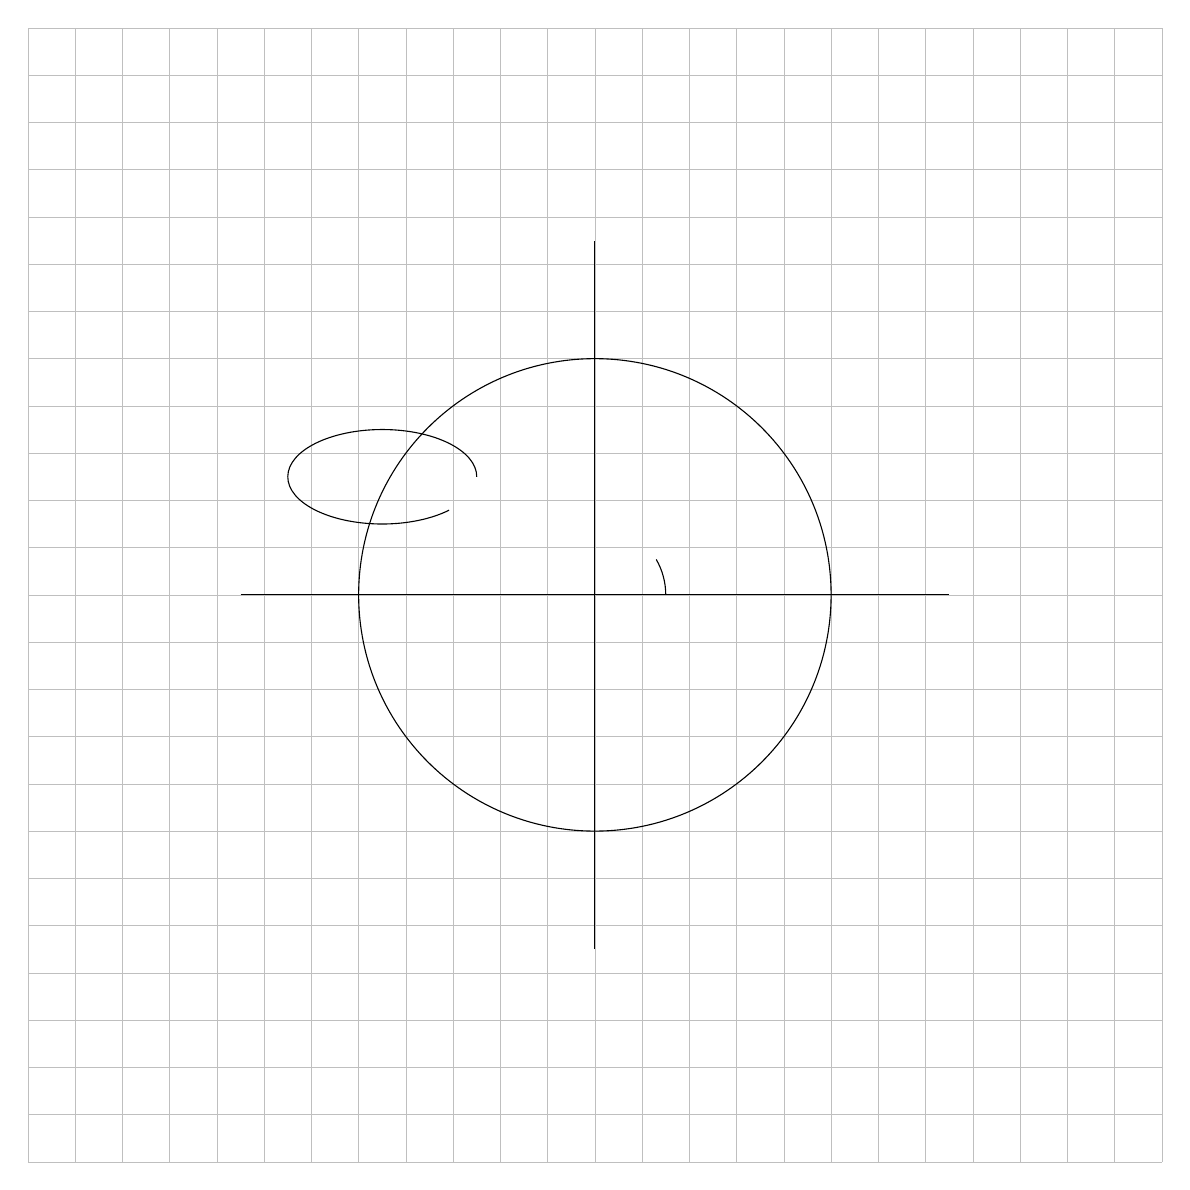
\begin{tikzpicture}[
      Karl's grid/.style ={help lines,step=0.2,color=#1!50},
      Karl's grid/.default=blue,
      scale=3]
    \draw[Karl's grid=gray] (-2.4,-2.4) grid (2.4,2.4);
    \draw (-1.5,0) -- (1.5,0);
    \draw (0,-1.5) -- (0,1.5);
    \draw (0,0) circle [radius=1cm];
    \draw (3mm,0) arc[radius=0.3cm, start angle=0, end angle=30];
    \draw (-0.5cm,0.5cm) arc[x radius=0.4cm, y radius=0.2cm, start angle=0, end angle=315];
    \end{tikzpicture}
  \end{center}
  \caption{}
  \label{fig:}
\end{figure}

\begin{figure}
  \begin{center}
    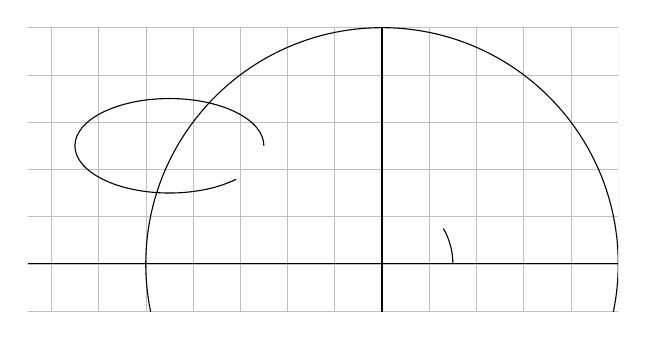
\begin{tikzpicture}[
      Karl's grid/.style ={help lines,step=0.2,color=#1!50},
      Karl's grid/.default=blue,
      scale=3]
    \clip (-1.5cm, -0.2cm) rectangle (1cm, 1cm);
    \draw[Karl's grid=gray] (-2.4,-2.4) grid (2.4,2.4);
    \draw (-1.5,0) -- (1.5,0);
    \draw (0,-1.5) -- (0,1.5);
    \draw (0,0) circle [radius=1cm];
    \draw (3mm,0) arc[radius=0.3cm, start angle=0, end angle=30];
    \draw (-0.5cm,0.5cm) arc[x radius=0.4cm, y radius=0.2cm, start angle=0, end angle=315];
    \end{tikzpicture}
  \end{center}
  \caption{}
  \label{fig:}
\end{figure}


\begin{figure}
  \begin{center}
    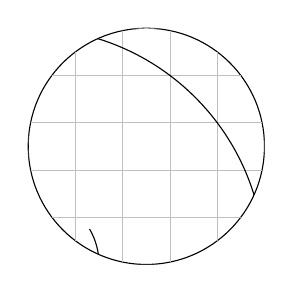
\begin{tikzpicture}[
      Karl's grid/.style ={help lines,step=0.2,color=#1!50},
      Karl's grid/.default=blue,
      scale=3]
    \clip[draw] (0.5cm, 0.5cm) circle (0.5cm);
    \draw[Karl's grid=gray] (-2.4,-2.4) grid (2.4,2.4);
    \draw (-1.5,0) -- (1.5,0);
    \draw (0,-1.5) -- (0,1.5);
    \draw (0,0) circle [radius=1cm];
    \draw (3mm,0) arc[radius=0.3cm, start angle=0, end angle=30];
    \draw (-0.5cm,0.5cm) arc[x radius=0.4cm, y radius=0.2cm, start angle=0, end angle=315];
    \end{tikzpicture}
  \end{center}
  \caption{}
  \label{fig:}
\end{figure}


\begin{figure}
  \begin{center}
    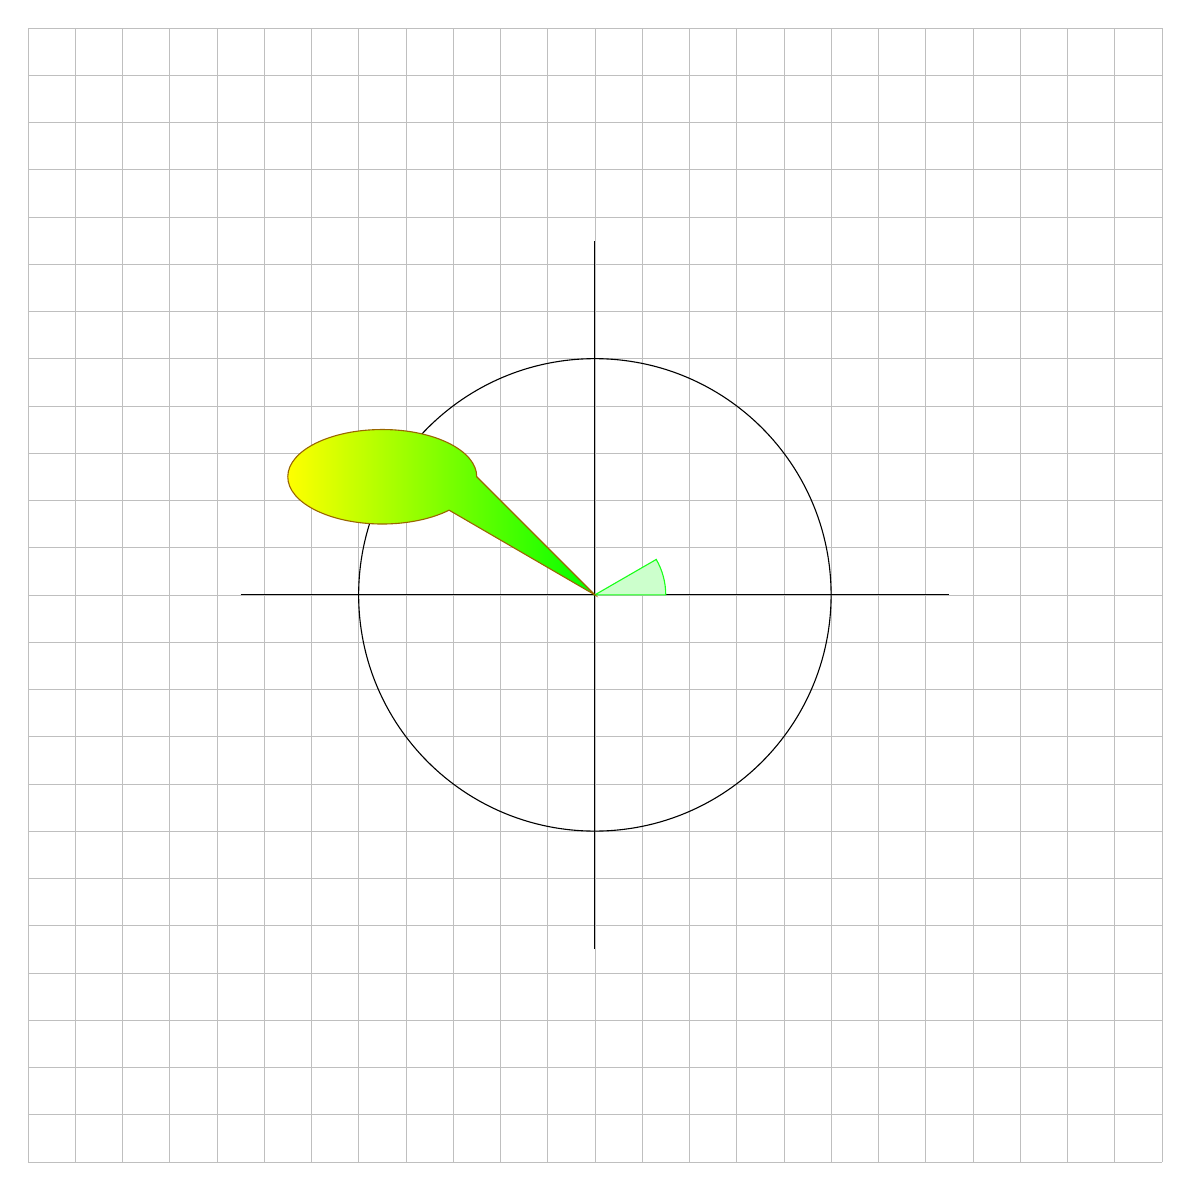
\begin{tikzpicture}[
      Karl's grid/.style ={help lines,step=0.2,color=#1!50},
      Karl's grid/.default=blue,
      scale=3]
    \draw[Karl's grid=gray] (-2.4,-2.4) grid (2.4,2.4);
    \draw (-1.5,0) -- (1.5,0);
    \draw (0,-1.5) -- (0,1.5);
    \draw (0,0) circle [radius=1cm];
    \filldraw[draw=green!90!white, fill=green!20!white] (0, 0) -- (3mm,0) arc[radius=0.3cm, start angle=0, end angle=30] -- cycle;
    %\filldraw[draw=red!60!green, fill=green!20!white] (0, 0) -- (-0.5cm,0.5cm) arc[x radius=0.4cm, y radius=0.2cm, start angle=0, end angle=315] -- cycle;

    \shadedraw[left color=yellow, right color=green, draw=red!60!green] (0, 0) -- (-0.5cm,0.5cm) arc[x radius=0.4cm, y radius=0.2cm, start angle=0, end angle=315] -- cycle;
    \end{tikzpicture}
  \end{center}
  \caption{}
  \label{fig:}
\end{figure}


\begin{figure}
  \begin{center}
    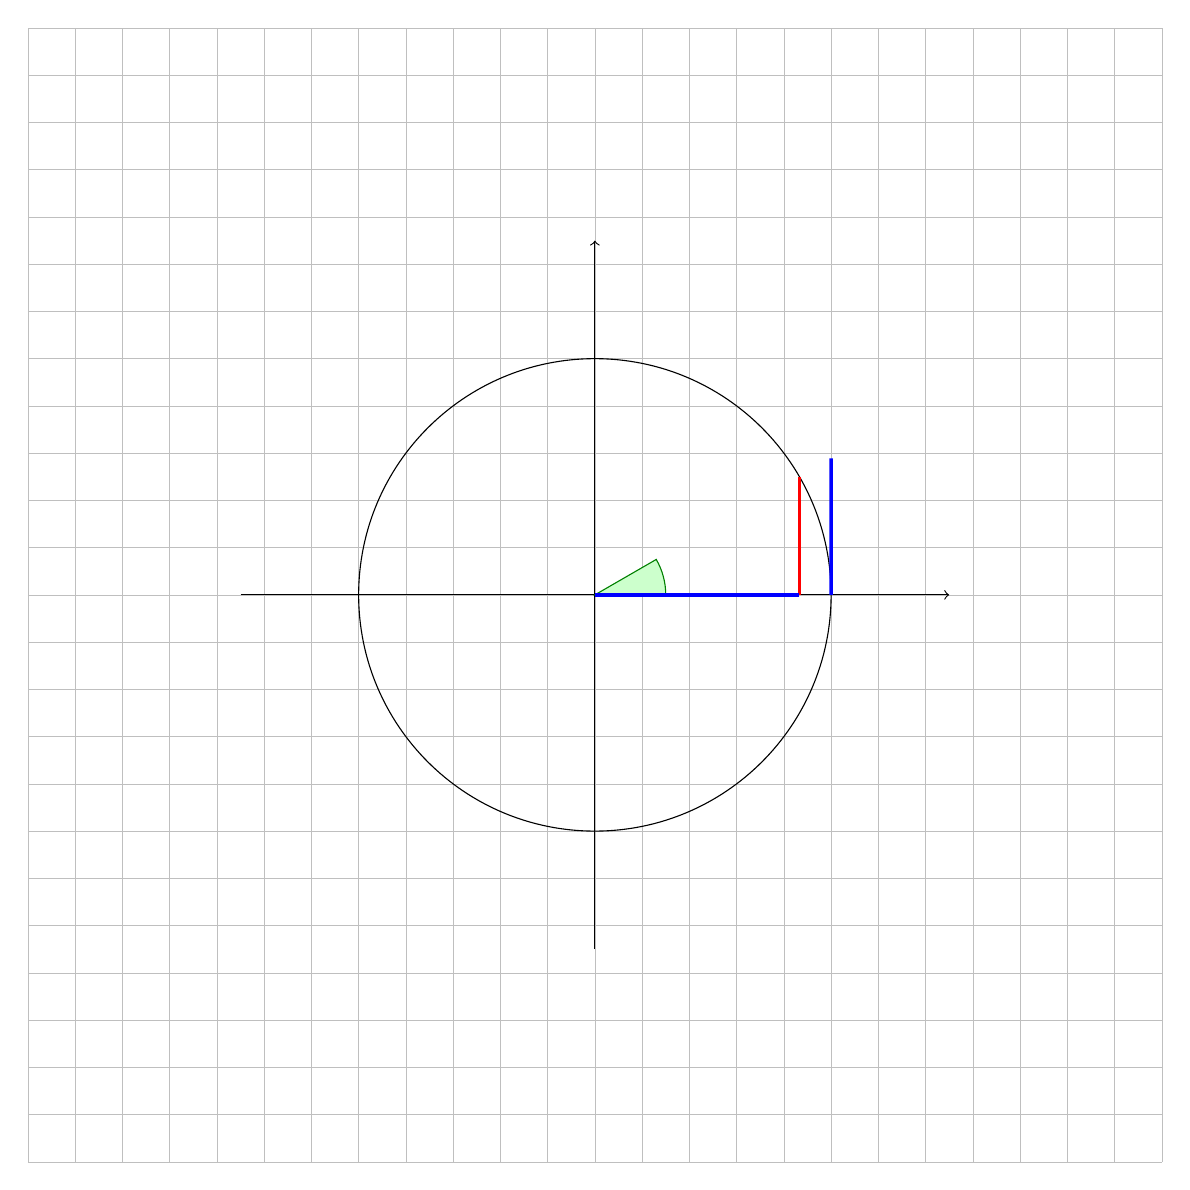
\begin{tikzpicture}[
      Karl's grid/.style ={help lines,step=0.2,color=#1!50},
      Karl's grid/.default=blue,
      scale=3
      ]
    \draw[Karl's grid=gray] (-2.4,-2.4) grid (2.4,2.4);
    \draw[->] (-1.5,0) -- (1.5,0);
    \draw[->] (0,-1.5) -- (0,1.5);
    \draw (0,0) circle [radius=1cm]; \filldraw[fill=green!20,draw=green!50!black] (0,0) -- (3mm,0mm)
    arc [start angle=0, end angle=30, radius=3mm] -- cycle; \draw[red,very thick] (30:1cm) -- +(0,-0.5); \draw[blue,very thick] (30:1cm) ++(0,-0.5) -- (0,0);
    \path [name path=upward line] (1,0) -- (1,1);
    \path [name path=sloped line] (0,0) -- (30:1.5cm); % a bit longer, so that there is an intersection
    % (add `\usetikzlibrary{intersections}' after loading tikz in the preamble)
    \draw [name intersections={of=upward line and sloped line, by=x}] [very thick,blue] (1,0) -- (x);
\end{tikzpicture}
  \end{center}
  \caption{}
  \label{fig:}
\end{figure}


\begin{figure}
  \begin{center}
    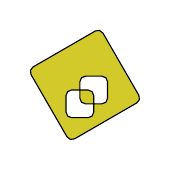
\begin{tikzpicture}[even odd rule,rounded corners=2pt,x=10pt,y=10pt]
    \filldraw[fill=yellow!80!black] (0,0) rectangle
      (1,1) [xshift=5pt,yshift=5pt] (0,0) rectangle (1,1)
                      [rotate=30] (-1,-1) rectangle (2,2);


    \end{tikzpicture}
      \end{center}
      \caption{}
  \label{fig:}
\end{figure}

% loop demo
\begin{figure}
  \begin{center}
    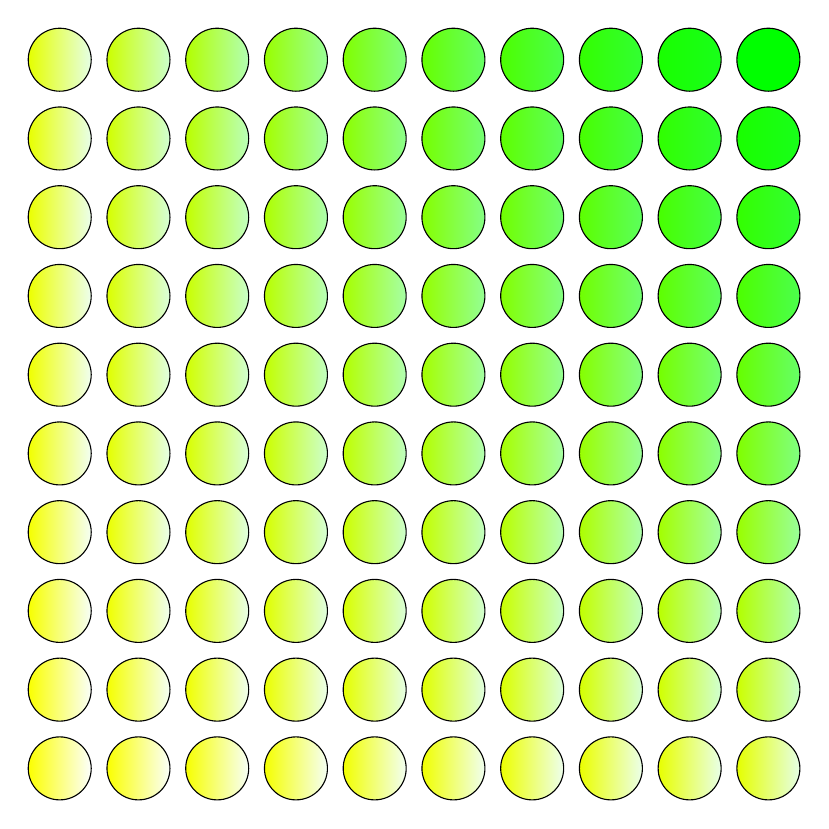
\begin{tikzpicture}[
    evaluate={
      int \i, \j;
      for \i in {0,...,10} {
        for \j in {0,...,10} {
          \a{\i,\j} = (\i*\j);
        };
      };
    }
  ]
      \foreach \x in {1, ..., 10}
        \foreach \y in {1, ..., 10}
        \shadedraw[left color=green!\a{\x,\y}!yellow, right color=green!\a{\y,\x}!white] (\x, \y) circle (0.4cm);
    \end{tikzpicture}
  \end{center}
  \caption{}
  \label{fig:}
\end{figure}

% loop demo
\begin{figure}
  \begin{center}
  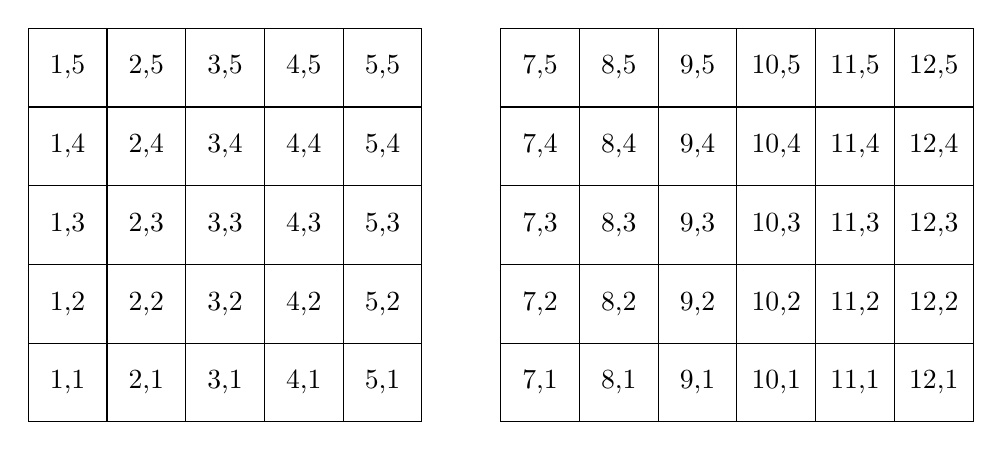
\begin{tikzpicture}
  \foreach \x in {1,2,...,5,7,8,...,12}
    \foreach \y in {1,...,5}
    {
      \draw (\x,\y) +(-.5,-.5) rectangle ++(.5,.5);
      \draw (\x,\y) node{\x,\y};
    }
 \end{tikzpicture}   
  \end{center}
  \caption{}
  \label{fig:}
\end{figure}


\begin{figure}
  \begin{center}
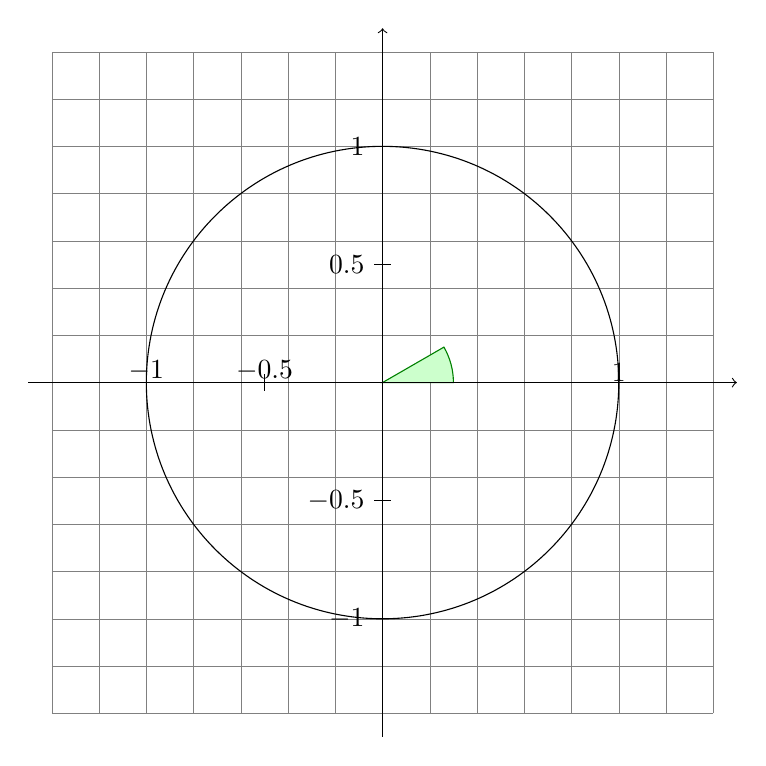
\begin{tikzpicture}[scale=3]
\draw[step=.2cm,color=gray!10!white,help lines] (-1.4,-1.4) grid (1.4,1.4);
\filldraw[fill=green!20,draw=green!50!black] (0,0) -- (3mm,0mm)
arc [start angle=0, end angle=30, radius=3mm] -- cycle;
\draw[->] (-1.5,0) -- (1.5,0);
\draw[->] (0,-1.5) -- (0,1.5);
\draw (0,0) circle [radius=1cm];
\foreach \x in {-1,-0.5,1}
  \draw (\x cm,1pt) -- (\x cm,-1pt) node[anchor=south] {$\x$};
\foreach \y in {-1,-0.5,0.5,1}
  \draw (1pt,\y cm) -- (-1pt,\y cm) node[anchor=east] {$\y$};
\end{tikzpicture}
  \end{center}
  \caption{}
  \label{fig:}
\end{figure}

\begin{figure}
  \begin{center}
    
\begin{tikzpicture}
   \node :fill opacity = { 0s="1", 2s="0", begin on=click }
         :rotate = { 0s="0", 2s="90", begin on=click }
         [fill = blue!20, draw = blue, ultra thick, circle] {Click me!};
    \end{tikzpicture}
  \end{center}
  \caption{}
  \label{fig:}
\end{figure}


% \tikz \graph [tree layout, sibling distance=1cm, nodes={circle,draw}] { 1--{2,3,4,5} };begin

% \begin{figure}
%   \begin{center}
% \tikz \graph [binary tree layout, sibling distance=4mm, level distance=8mm, components go right top aligned,
% component sep=1pt, nodes=draw]
% {
%   1 -> 2 -> {3->4[second]->5,6,7};
%   a -> b[second] -> c[second] -> d -> e;
%   x -> y[second] -> z -> u[second] -> v;
% };
%   \end{center}
%   \caption{}
%   \label{fig:}
% \end{figure}


% \begin{figure}
% \begin{tikzpicture}
% \graph [simple necklace layout, node distance=1cm, node sep=0pt,
% nodes={draw,circle,as=.}] {
% 1 -- 2 [minimum size=2cm] -- 3 --
% 4 -- 5 -- 6 -- 7 --[orient=up] 8 };
%   \draw [red,|-|] (1.center) -- ++(0:1cm);
%   \draw [red,|-|] (5.center) -- ++(180:1cm);
% \end{tikzpicture}\end{figure}

\end{document}
